\documentclass[a4paper,11pt]{ltjsarticle}
\usepackage{graphicx}
\usepackage{luatexja-fontspec}
\usepackage{caption}
\usepackage{amsmath,amssymb,bm,braket}
\usepackage[english]{babel}
\usepackage{multicol}
\usepackage{titlesec}
%\usepackage{gnuplot-lua-tikz}
\usepackage[top=20truemm,bottom=20truemm,left=20truemm,right=20truemm]{geometry}
\usepackage{array}
\usepackage{upgreek}
\usepackage{fancyhdr}
\renewcommand{\refname}{}
\usepackage{listings,jvlisting}
\usepackage{tikz}
\usepackage[thmmarks,amsmath]{ntheorem}
\usepackage[version=3]{mhchem}
\usetikzlibrary{external}
\tikzexternalize
\lstset{
  basicstyle={\ttfamily},
  identifierstyle={\small},
  commentstyle={\smallitshape},
  keywordstyle={\small\bfseries},
  ndkeywordstyle={\small},
  stringstyle={\small\ttfamily},
  frame={tb},
  breaklines=true,
  columns=[l]{fullflexible},
  numbers=left,
  xrightmargin=0pt,
  xleftmargin=3pt,
  numberstyle={\scriptsize},
  stepnumber=1,
  numbersep=1pt,
  lineskip=-0.5ex
}
\captionsetup[figure]{format=plain, labelformat=simple, labelsep=quad,labelfont=bf,name={Fig.}}
\captionsetup[table]{format=plain, labelformat=simple, labelsep=quad,labelfont=bf}
\parindent = 0pt
%[BoldFont=HGSMinchoE]{MSMincho}[BoldFont=HiraMinProN-W6]{HiraMinPro-W3}
\titleformat{\section}{\normalfont\fontsize{9}{10}\bfseries\fontspec{Times New Roman}}{\thesection.}{1em}{}
\usepackage[backend=biber,sorting=none,style=numeric,maxnames=99,minnames=1]{biblatex}
\addbibresource{utility/REFERENCES.bib}
\defbibheading{bibliography}[\refname]{%
  \section*{REFERENCES}%
  \vspace{-7pt}  % ここで空白を調整。お好みの値に変更してください。
}
\newfontfamily\subsectionfont{Times New Roman} % サブセクション用フォント
\titleformat{\subsection}
  {\normalfont\large\bfseries} % サブセクションのフォントを指定
  {\thesubsection}{1em}{}
\renewbibmacro{in:}{}
\renewbibmacro*{journal+issuetitle}{%
  \addcomma\space% カンマとスペースを追加
  \usebibmacro{journal}%
  \setunit*{\addspace}%
  \usebibmacro{volume+number+eid}%
  \setunit{\addspace}%
  \printfield{note}%
  \newunit
}
\renewbibmacro*{volume+number+eid}{
  \printfield{volume}%
  \setunit*{\addnbspace}%
  \printfield{number}%
  \setunit{\addcomma\space}%
  \printfield{eid}
}
\DeclareFieldFormat[article]{volume}{\textbf{#1}}
\DeclareFieldFormat[article]{pages}{#1}
\DeclareFieldFormat{journaltitle}{#1}
\usepackage{hyperref}
\renewenvironment{abstract}{\par\noindent}{\par}
%\pagenumbering{gobble}
\usepackage{docmute}
\usepackage{setspace}
\usepackage{titlesec} % 見出しのカスタマイズ用

% セクションのフォーマットをカスタマイズ
\titleformat{\section}
  {} % フォントサイズとスタイル
  {\Large\bfseries\thesection\ \ }               % 番号の前の内容(空白)
  {0em}            % 番号とタイトルの間の間隔
  {\Large\bfseries}


\theoremstyle{plain}
\theoremheaderfont{\normalfont\bfseries}
\theorembodyfont{\itshape}   % 本文を斜体に
\theoremseparator{.}         % タイトルと本文の区切りを「.」に設定
\newtheorem{definition}{Definition}
\begin{document}
\section{Stabilizer Formalism \cite{nielsen2010}}{
    \ \ \ In this section, we describe the stabilizer formalism, which forms the backbone of quantum error correction theory. Before delving into the main discussion, we provide a small case example of error correction and briefly introduce classical error correction theory.
    \subsection{Introduction to Error Correction}\label{introduction_to_error_correction}{
        \ \ \ Noise is a great bane of information systems. Whenever we build systems for computation or other purposes, we cannot avoid noise from outside the system. However, even in such environments, classical components perform reliable computation with a failure rate typically below one error in $10^{17}$ operations. The details of the techniques used to protect against noise in practice are sometimes rather complicated, but the basic principles are easily understood. For example, consider the case when Alice sends Bob a single bit of information through a noisy channel, where the error rate is $p$. If Alice sends a bit without protection, a bit-flip error, where $0$ flips to $1$ and vice versa, occurs with a probability of $p$. As a result, Bob will fail to receive the correct information from Alice with a probability of $p$. In such cases, we cannot communicate reliably through the noisy channel. Yet, there is a way to address this issue. If Alice introduces redundancy for a bit of information, a process called "encoding," such as:

        \begin{align}
            0 \rightarrow 000 \quad \text{or} \quad 1 \rightarrow 111,
        \end{align}      
        Then Alice uses 2 additional bits to send a single bit of information, effectively using two additional channels. In this case, assume Alice sends $000$. Each bit can be flipped with a probability of $p$. Bob then receives:
        \begin{itemize}
            \item No bit flipped, e.g., $000$, with a probability of $(1-p)^3$,
            \item One bit flipped, e.g., $100$, $010$, $001$, with a probability of $3p(1-p)^2$,
            \item Two bits flipped, e.g., $110$, $101$, $011$, with a probability of $3p^2(1-p)$,
            \item Three bits flipped, e.g., $111$, with a probability of $p^3$.
        \end{itemize}
        Thus, Bob will receive $000$, $100$, $010$, or $001$ with a probability of $(1-p)^3 + 3p(1-p)^2$. He then performs a majority vote between $0$ and $1$, allowing him to restore the information sent by Alice. For reliable communication through encoding, the probability of failure, $3p^2(1-p) + p^3$, must be less than $1/2$. This gives the threshold for reliable communication as $p < 1/2$. Encoding a bit of information into several bits by repeating the original is called a repetition code.

        \subsection{Error Correction Beyond Classical Ones}\label{repetition_code}{
            \ \ \ In quantum environments, we cannot perform error correction in the same way as described in Section \ref{introduction_to_error_correction}, because performing a majority vote on an encoded qubit destroys the qubit state, collapsing it into one of the eigenstates of the observable. This is crucial, as in quantum computation, we cannot ignore noise while performing operations. We need to correct errors and perform computational operations simultaneously. If we destroy the states of qubits, we cannot continue the remaining computation. There are also important differences between classical information and quantum information, requiring new ideas to make quantum error-correcting codes possible. In particular, at first glance, we encounter three rather formidable difficulties to address \cite{nielsen2010}:

            \begin{itemize}
                \item \textit{No cloning}: One might try to implement the repetition code quantum mechanically by duplicating the quantum state three or more times. This is forbidden by the no-cloning theorem.
                \item \textit{Errors are continuous}: A continuum of different errors may occur on a single qubit.
                Determining which error occurred in order to correct it would appear to require infinite precision, and therefore infinite resources.
                \item \textit{Measurement destroys quantum information}: In classical error-correction we observe the output from the channel, and decide what decoding procedure to adopt. Observation in quantum mechanics generally destroys the quantum state under observation, and makes recovery impossible.
            \end{itemize}

            Fortunately, these difficulties are not fatal, and we will demonstrate a quantum version of the repetition code to illustrate this. In quantum error correction, there exist two types of errors, in contrast to classical computation: bit-flip errors and phase-flip errors. Bit-flip errors are the same as those in classical computation; for example, they are represented as $X\ket{\psi}$. Phase-flip errors occur when some qubits are acted on by $Z$, such as $Z\ket{\psi}$. from dualiality of X and Z, we only consider the case that bit-flip errors, and the case of phase-flip errors we can apply the same way as bit-flip. In this demonstration, we will demonstrate the repetition code for bit-flip errors. 
            \ \ \ Suppose we encode the state \(\ket{\phi} = a\ket{0} + b\ket{1}\) into a three-qubit space as \(\ket{\psi} = a\ket{000} + b\ket{111}\). A useful way to express this is:

            \begin{align}
                    \ket{0}_L \rightarrow \ket{000},\ \ \ \ket{1}_L \rightarrow \ket{111}.
            \end{align}

            Here, \(\ket{\cdot}_L\) is called the "logical qubit," while \(\ket{\cdot}\) is called the "physical qubit." In this encoding scheme, we now obtain the encoding circuit shown below in Fig.~\ref{encoding_repetition}.

            \begin{figure}[h]
                \centering
                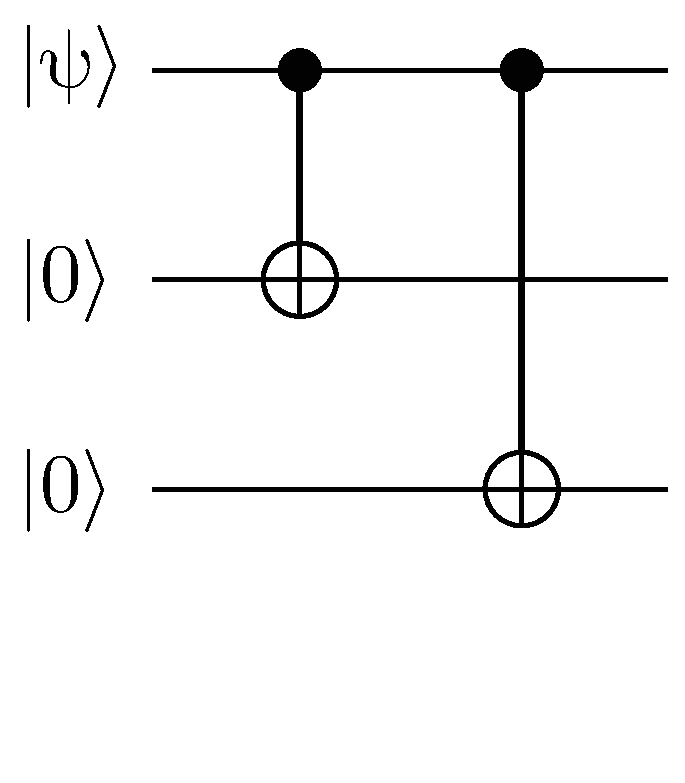
\includegraphics[scale=0.40]{figure/encoding_repetition.eps}
                \vspace{-40pt}\caption{}
                \label{encoding_repetition}
                \vspace{-15pt}
            \end{figure}

            Using the encoded state, we can obtain syndromes that indicate where an error has occurred. In this code, these syndromes can be determined by performing Pauli measurements of $Z_1 Z_2$ and $Z_2 Z_3$. For example, when no error has occurred on \(\ket{\psi}\), we will obtain syndromes of $1$ and $1$ from $Z_1 Z_2$ and $Z_2 Z_3$, respectively, due to a straightforward calculation:
            
            \begin{align*}
                Z_1Z_2\ket{\psi} &= aZ_1Z_2\ket{000}+bZ_1Z_2\ket{111}\\
                &= a\ket{000}+b\ket{111}\\
                &= \ket{\psi}
            \end{align*}
            \begin{align*}
                Z_2 Z_3\ket{\psi} &= aZ_2Z_3\ket{000}+bZ_2Z_3\ket{111}\\
                &= a\ket{000}+b\ket{111}\\
                &= \ket{\psi}
            \end{align*}

            However, if an error has occurred on the first qubit of the three, we will obtain syndromes of $-1$ and $1$ from $Z_1 Z_2$ and $Z_2 Z_3$, respectively, due to a straightforward calculation:

            \begin{align*}
                Z_1Z_2\ket{\psi} &= aZ_1Z_2\ket{100}+bZ_1Z_2\ket{011}\\
                &= -a\ket{100}-b\ket{011}\\
                &= -\ket{\psi}
            \end{align*}
            \begin{align*}
                Z_2 Z_3\ket{\psi} &= aZ_2Z_3\ket{100}+bZ_2Z_3\ket{011}\\
                &= a\ket{100}+b\ket{011}\\
                &= \ket{\psi}.
            \end{align*}

            Thus, we can determine that a bit-flip error has occurred on the first qubit and correct the error. In this case, we can correct a single error on any qubit. However, we cannot correct two or three errors. For instance, in the case of two errors on the second and third qubits of the three, we will obtain the following syndromes:

            \begin{align*}
                Z_1Z_2\ket{\psi} &= aZ_1Z_2\ket{011}+bZ_1Z_2\ket{100}\\
                &= -a\ket{011}-b\ket{100}\\
                &= -\ket{\psi}
            \end{align*}
            \begin{align*}
                Z_2 Z_3\ket{\psi} &= aZ_2Z_3\ket{011}+bZ_2Z_3\ket{100}\\
                &= a\ket{110}+b\ket{100}\\
                &= \ket{\psi}.
            \end{align*}

            These syndromes are the same as in the former case, so we cannot determine whether a single error has occurred on the first qubit or two errors have occurred on the second and third qubits. in the case of three errors, we will obtain the following syndromes:

            \begin{align*}
                Z_1Z_2\ket{\psi} &= aZ_1Z_2\ket{111}+bZ_1Z_2\ket{000}\\
                &= a\ket{111}+b\ket{000}\\
                &= \ket{\psi}
            \end{align*}
            \begin{align*}
                Z_2 Z_3\ket{\psi} &= aZ_2Z_3\ket{111}+bZ_2Z_3\ket{000}\\
                &= a\ket{111}+b\ket{000}\\
                &= \ket{\psi},
            \end{align*}

            which makes it appear as though no errors have occurred, even though errors have actually occurred. In summary, this code can detect and correct one error, can detect two errors but cannot correct them, and cannot detect or correct three errors.\\
            \ \ \ One may find that if a continuous error, such as $\ket{0} \rightarrow \ket{0} + \ket{1}$, occurs, we cannot obtain syndromes. Actually, when we obtain syndromes, we perform syndrome measurements using $Z_1 Z_2$ and $Z_2 Z_3$. As a result, the superposition state will be projected to either $\ket{0}$ or $\ket{1}$ with a probability proportional to the coefficients of the superposition state.\\
            \ \ \ In the following section, we refer to the minimum number of errors that cannot be detected as the code distance, often expressed as $d$, encoded qubits as logical qubits, and the number of them as $k$, and qubits used to encode logical qubits as physical qubits, with their number often expressed as $n$. The properties of the code are often denoted as $[[n, k, d]]$. In the case of the former repetition code, its properties are $[[3, 1, 1]]$, but this code cannot correct phase-flip errors. Therefore, we show how to correct both types of errors: bit-flip and phase-flip.
        }

        \subsection{Stabilizer}{
            \ \ \ Stabilizer formalism is the most fundamental concept in quantum error correction. The stabilizer group is denoted as $\mathcal{S}$, and its elements are Pauli matrices, so $\mathcal{S} \subseteq \mathcal{P}$, but $-I \not\in \mathcal{S}$. We also define the centralizer $\mathcal{C(S)}$, whose elements are Pauli matrices that commute with all elements of $\mathcal{S}$. Unlike classical codes, quantum codes are designed for computation while correcting errors, so there exist logical operators that change the states of logical qubits but leave stabilizer states unchanged. These logical operators $L$ exist in $\mathcal{C(S)} \backslash \mathcal{S}$. In the context of Section \ref{repetition_code}, $\mathcal{S} = \{Z_1Z_2, Z_2Z_3\}$ and $\mathcal{C(S)} = \{Z_1, Z_2, Z_3, X_1X_2X_3\}$, so in this case, the logical operators are $L_X = X_1X_2X_3$ and $L_Z = Z_1$, $Z_2$, or $Z_3$. As a side note, $Z_1$, $Z_2$, and $Z_3$ are equivalent logical operators in the quotient group of the stabilizer group.\\
            \ \ \ In quantum error correction theory, there are representative codes, and we will provide an example of one, called the Steane Code \cite{steane1996}. The Steane Code consists of 7 qubits and 6 stabilizer generators, making it an $[[7, 1, 1]]$ code. Stabilizer generators form the basis of the stabilizer group, meaning all elements of the stabilizer group can be expressed as products of stabilizer generators. stabilizer generators and logical operators are shown in Tab. \ref{steane_code}.

            \begin{table}[h]
                \centering
                \caption{ }
                \label{steane_code}
                \begin{tabular}{cc}
                    \hline
                    Stabilizer Generators & Logical Operators\\
                    \hline
                    {\setlength{\arraycolsep}{1pt}
                    $\begin{array}{ccccccc}
                        I&I&I&X&X&X&X\\
                        I&X&X&I&I&X&X\\
                        X&I&X&I&X&I&X\\
                        I&I&I&Z&Z&Z&Z\\
                        I&Z&Z&I&I&Z&Z\\
                        Z&I&Z&I&Z&I&Z
                    \end{array}$}&{\setlength{\arraycolsep}{1pt}
                    $\begin{array}{cccccccc}
                        L_X=&X&X&X&X&X&X&X\\
                        L_Z=&Z&Z&Z&Z&Z&Z&Z
                    \end{array}$}\\
                    \hline
                \end{tabular}
            \end{table}

            One may wonder how to encode a logical qubit in such codes. Encoding involves preparing a stabilizer state for the encoded qubits, so all you need to do is perform projective measurements of the stabilizer generators. First, you initialize all physical qubits to $\ket{0}$. This state is already a stabilizer state of the $Z$ stabilizers listed in Tab.~\ref{steane_code}. Second, you only need to perform projective measurements of the $X$ stabilizers. Consequently, the encoded state $\ket{0}_L$ can be expressed as follows:
            \begin{align*}
                \ket{0}_L=\prod_{i}(I+s_i)\ket{0000000}
            \end{align*}
            where $s_i$ is a $Z$ stabilizer generator, and the state is post-selected to the $+1$ eigenstates, ignoring the normalization factor. In the same way, $\ket{1}_L$ can be encoded. Thus, if you want to encode an arbitrary state $\ket{\psi} = a\ket{0} + b\ket{1}$, first prepare the Bell state $a\ket{0000000} + b\ket{1111111}$ and perform projective measurements of the $Z$ stabilizer generators. The final states is:

            \begin{align*}
                \ket{\psi_L}=\prod_{i}(I+s_i)\ket{0000000}+\prod_{i}(I+s_i)\ket{1111111}.
            \end{align*}

            From straightforward calculations, you can confirm that $L_X\ket{0}_L = \ket{1}_L$, $L_Z\ket{1}_L = -\ket{1}_L$, and $L_XL_Z = -L_ZL_X$. By definition, a logical operator cannot be expressed as the product of stabilizer generators.



        }
        



    }
}
\end{document}